\begin{center}
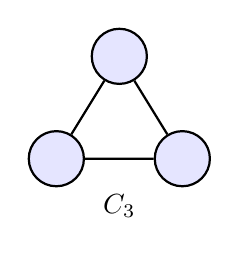
\begin{tikzpicture}[
  vnode/.style={circle, draw, minimum size=7mm, inner sep=0pt, fill=blue!10},
  thick
]
  \node[vnode] (r1) at (0, 0.9) {};
  \node[vnode] (r2) at (-0.8, -0.4) {};
  \node[vnode] (r3) at (0.8, -0.4) {};
  
  \draw (r1) -- (r2) -- (r3) -- (r1);
  
  \node at (0, -1.0) {$C_3$};
\end{tikzpicture}

\par\medskip
\textit{Obrázek 3.6: Příklad 2-regulárního grafu $C_3$.}
\end{center}